\section{Risultati}
In questa sezione di relazione verranno esposti i risultati restituiti dal HEC-RAS.\\
Grazie alle sezioni di profilo \eqref{figure:profili}, è possibile ricavare il massimo andamento del flusso dell'evento. Inoltre, mediante la funzione simil-gis di RasMapper, è possibile interrogare i singoli layer e ricavare i valori puntuali per ogni punto interno al dominio di calcolo.

\subsection{Flusso transitato nel fiume Boite e Piave}
I diagramma di velocità e profondità del tirante sono riportati successivamente nelle figure \eqref{figure:depth_boite}\eqref{figure:velocity_boite}\eqref{figure:depth_piave}\eqref{figure:velocity_piave}.\\
I profili utilizzati sono quelli denominati ``profilo\textunderscore boite" e ``profilo\textunderscore piave".

\begin{figure}[H] \centering
    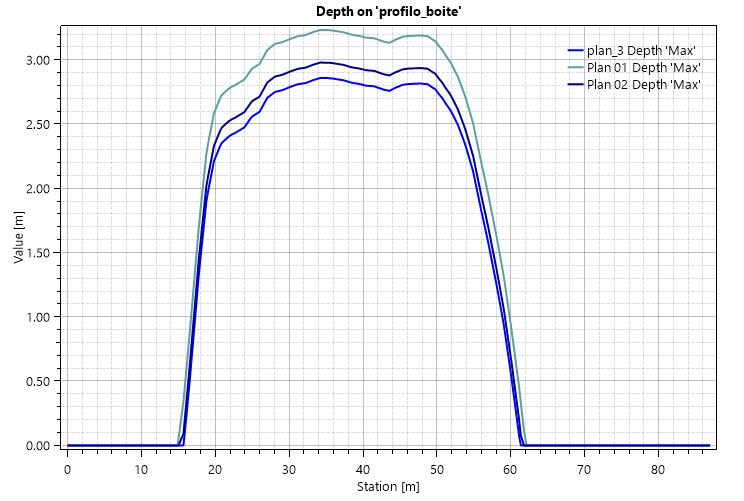
\includegraphics[scale=0.5]{immagini/depth_boite.JPG}
    \caption{Andamento del tirante idraulico, durante l'evento di piena, nel fiume Boite.}
    \label{figure:depth_boite}
\end{figure}

\begin{figure}[H] \centering
    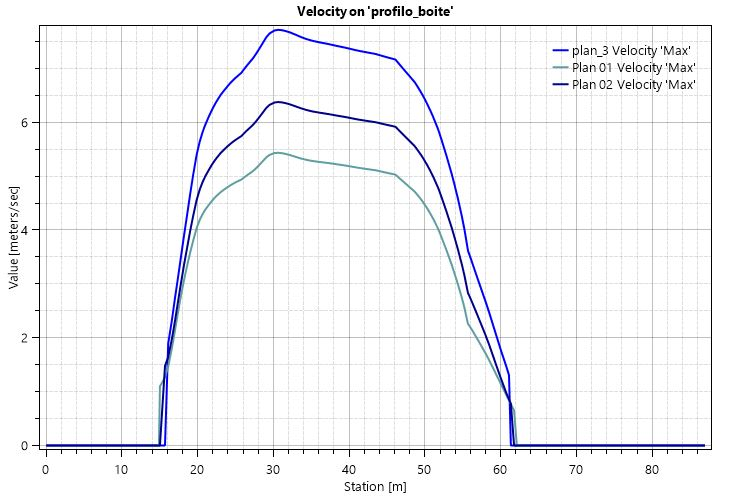
\includegraphics[scale=0.5]{immagini/velocity_boite.JPG}
    \caption{Andamento della velocità di flusso, durante l'evento di piena, nel fiume Boite.}
    \label{figure:velocity_boite}
\end{figure}

\begin{figure}[H] \centering
    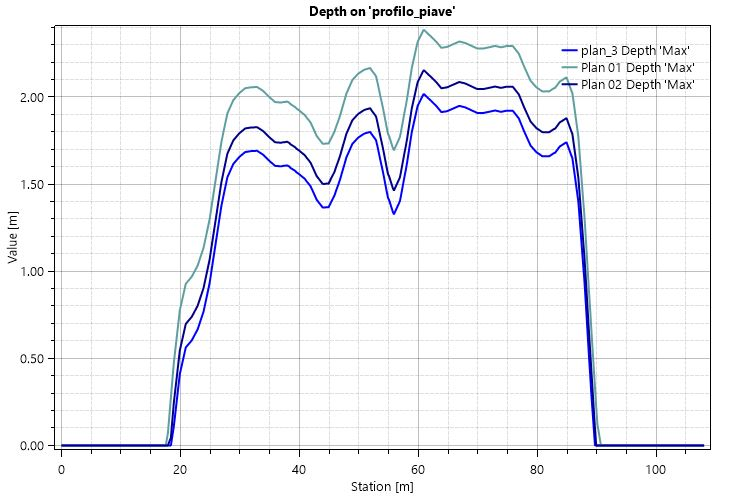
\includegraphics[scale=0.5]{immagini/depth_piave.JPG}
    \caption{Andamento del tirante idraulico, durante l'evento di piena, nel fiume Piave.}
    \label{figure:depth_piave}
\end{figure}

\begin{figure}[H] \centering
    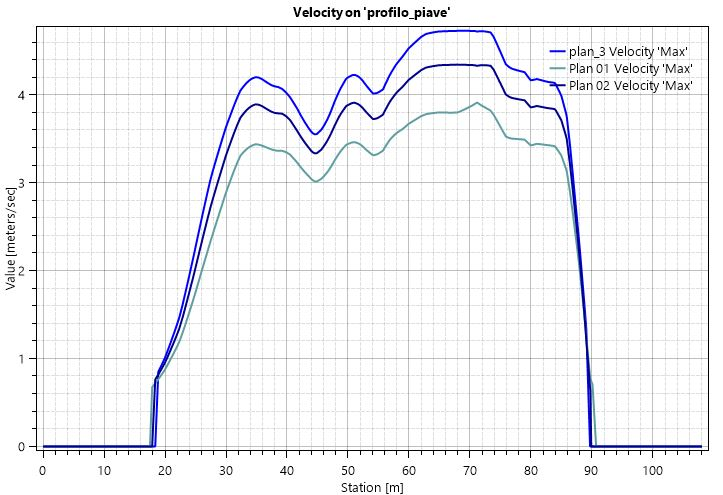
\includegraphics[scale=0.5]{immagini/velocity_piave.JPG}
    \caption{Andamento della velocità di flusso, durante l'evento di piena, nel fiume Piave.}
    \label{figure:velocity_piave}
\end{figure}

E' interessante notare la differenza tra l'andamento della velocità del fiume Piave \eqref{figure:velocity_piave} e del fiume Boite \eqref{figure:velocity_boite}: quest'ultima ha una maggiore omogeneità di valori massimi rispetto alla prima; tale caratteristica è dovuta alla differente geometria del letto dell'alveo.

\subsection{Flusso in uscita dal dominio}
In questa sottosezione verranno esposti i risultati della simulazione nel tratto a valle dell'abitato, in prossimità dell'uscita dal dominio di calcolo.\\
Il profilo da cui sono stati ricavati gli idrogrammi è stato denominato  ``profilo\textunderscore piave\textunderscore outflow".\\
I diagrammi risultanti sono \eqref{figure:depth_piave_outflow}\eqref{figure:velocity_piave_outflow}.

\begin{figure}[H] \centering
    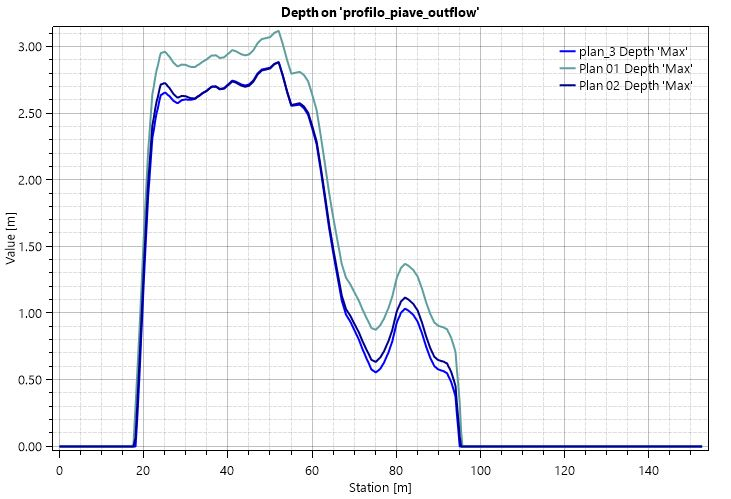
\includegraphics[scale=0.5]{immagini/depth_piave_outflow.JPG}
    \caption{Andamento del tirante idraulico, durante l'evento di piena, nel tratto finale del fiume Piave.}
    \label{figure:depth_piave_outflow}
\end{figure}

\begin{figure}[H] \centering
    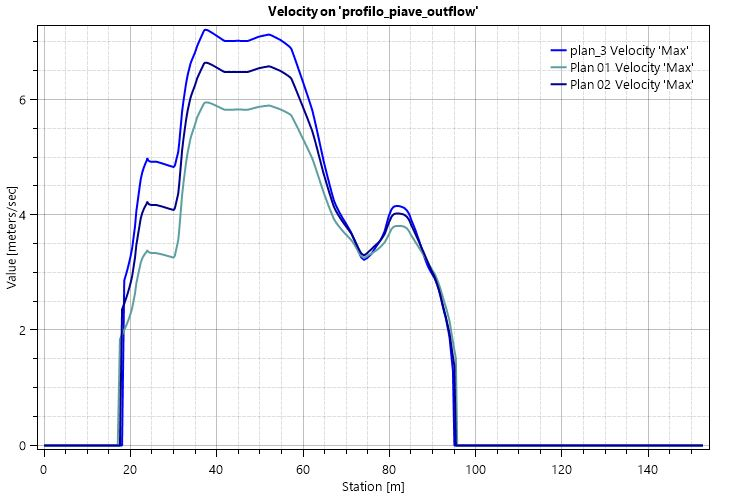
\includegraphics[scale=0.5]{immagini/velocity_piave_outflow.JPG}
    \caption{Andamento della velocità di flusso, durante l'evento di piena, nel tratto finale del fiume Piave.}
    \label{figure:velocity_piave_outflow}
\end{figure}

I risultati sono concordi con quanto previsto: per la simulazione con un Manning relativamente maggiore (ovvero ``plan\textunderscore 1"), la profondità del tirante è maggiore rispetto alle altre due simulazioni. Lo stesso ragionamento può essere fatto con le velocità: il risultato della simulazione con un valore di Manning inferiore agli altri due (ovvero ``plan\textunderscore 3") ha restituito una velocità del flusso ben superiore agli altri due casi.

\subsection{Andamento in prossimità dei ponti}
Lo studio del cinematismo in prossimità del ponte può risultare utile per studiare i possibili casi di rigurgito \cite{rigurgito}.\\
Per quanto riguarda la criticità idraulica che i ponti rappresentano, risulta utile tenere in considerazione l'andamento del cappio di piena dell'evento di deflusso. Purtroppo, per tutte le sezioni disegnate all'interno del dominio di calcolo, i diagrammi plottati da HEC-RAS non sono risultati utili per ricavarne delle informazioni, perché sono troppo distorti.\\
Essendoci due ponti, i profili individuati in alveo sono 4: uno a monte ed uno a valle per ciascuno \eqref{figure:depth_monte_ponte_boite}\eqref{figure:depth_valle_ponte_boite}\eqref{figure:depth_monte_ponte_piave}\eqref{figure:depth_valle_ponte_piave}.

\begin{figure}[H] \centering
    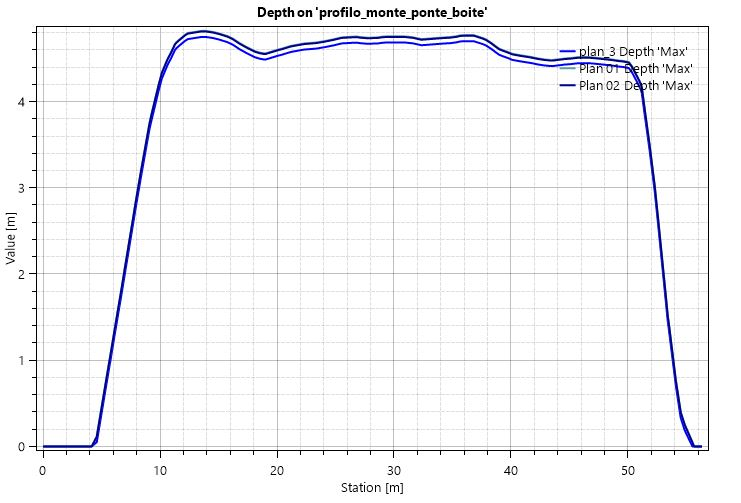
\includegraphics[scale=0.5]{immagini/depth_monte_ponte_boite.JPG}
    \caption{Andamento del tirante idraulico, durante l'evento di piena, a monte del ponte nel fiume Boite.}
    \label{figure:depth_monte_ponte_boite}
\end{figure}

\begin{figure}[H] \centering
    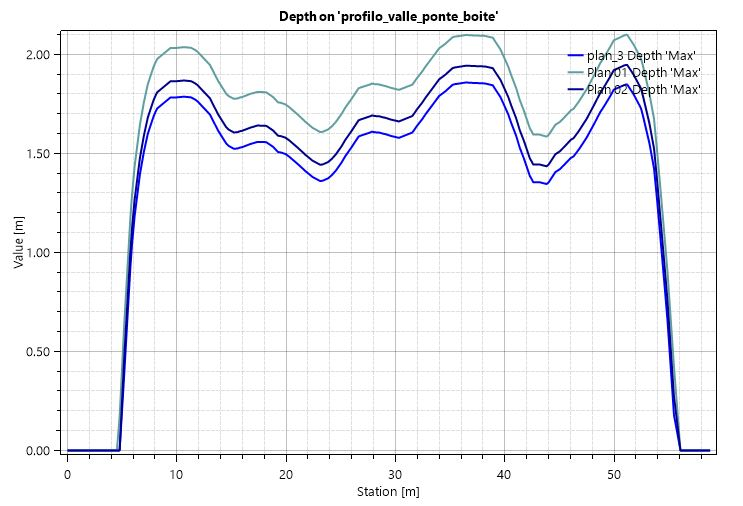
\includegraphics[scale=0.5]{immagini/depth_valle_ponte_boite.JPG}
    \caption{Andamento del tirante idraulico, durante l'evento di piena, a valle del ponte nel fiume Boite.}
    \label{figure:depth_valle_ponte_boite}
\end{figure}

\begin{figure}[H] \centering
    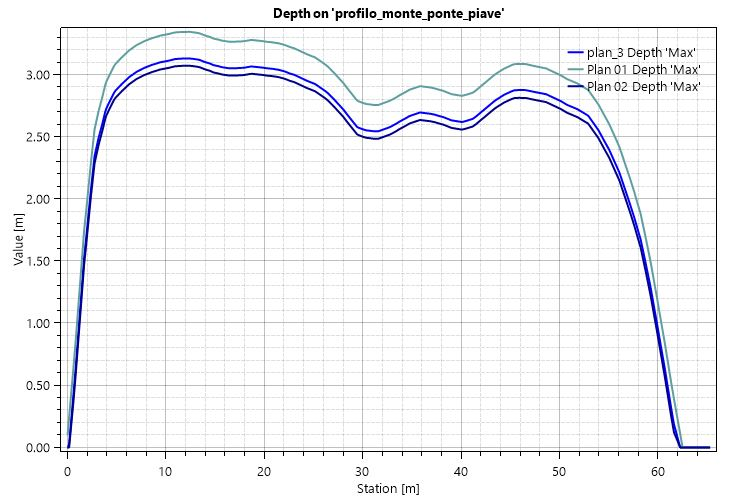
\includegraphics[scale=0.5]{immagini/depth_monte_ponte_piave.JPG}
    \caption{Andamento del tirante idraulico, durante l'evento di piena, a monte del ponte nel fiume Piave.}
    \label{figure:depth_monte_ponte_piave}
\end{figure}

\begin{figure}[H] \centering
    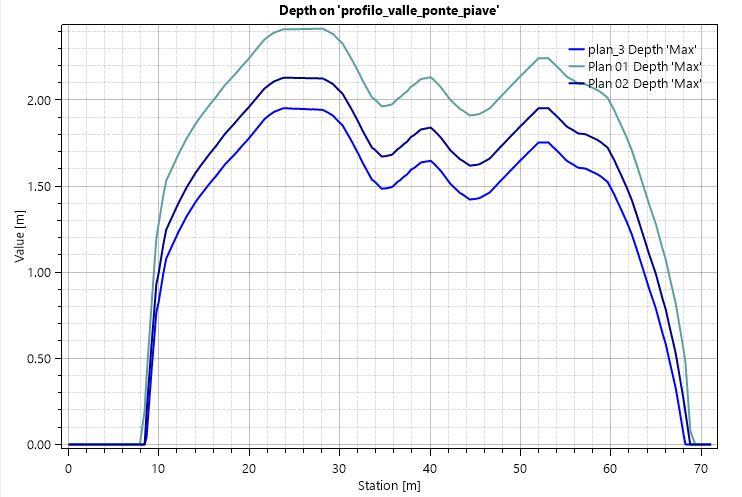
\includegraphics[scale=0.5]{immagini/depth_valle_ponte_piave.JPG}
    \caption{Andamento del tirante idraulico, durante l'evento di piena, a valle del ponte nel fiume Piave.}
    \label{figure:depth_valle_ponte_piave}
\end{figure}

Anche in questo caso, è possibile notare come la profondità del corso d'acqua sia maggiore per l'evento di piena con i valori di Manning maggiori (come per esempio la prima simulazione).

\subsection{Flusso transitato sotto i ponti}
Utilizzando la funzione di HEC-RAS, denominata ``Plot Stage and Flow Hydrograph", è possibile ricavare l'idrogramma di deflusso dell'evento (e quindi anche la portata) che attraversa le luci dei ponti presenti in alveo.\\
Solamente per esempio, si riportano i diagrammi di deflusso (uno per ciascun ponte) della terza simulazione, ovvero quella con valore di Manning inferiore rispetto alle altre due. 
\begin{figure}[H] \centering
    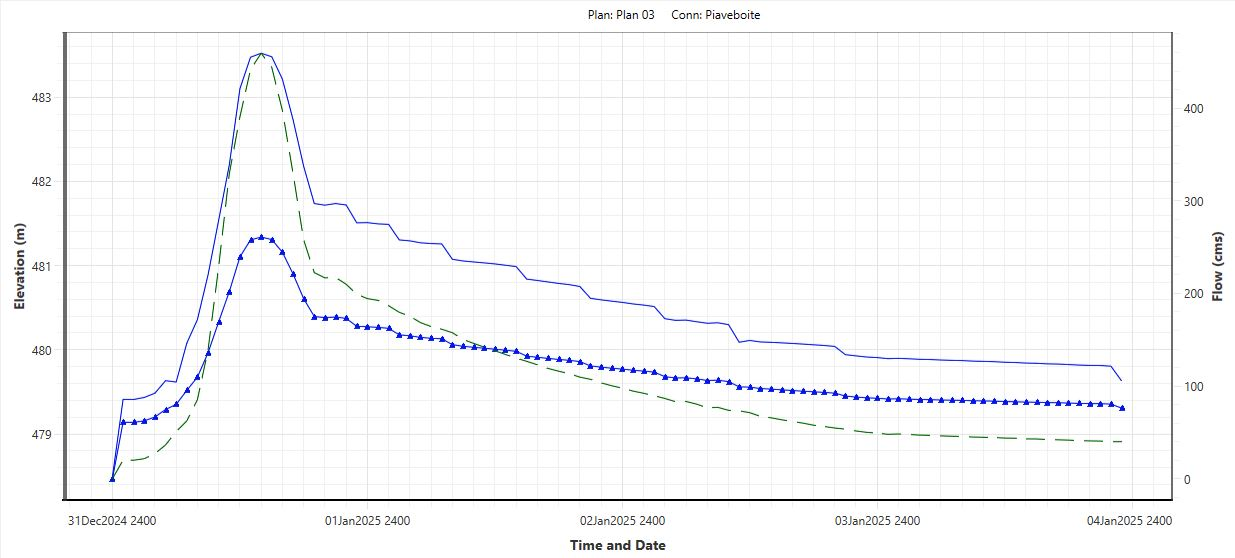
\includegraphics[scale=0.5]{immagini/flow_ponte_boite.JPG}
    \caption{Portata di deflusso transitata al di sotto del ponte nel fiume Boite, calcolata con la terza simulazione.}
    \label{figure:flow_ponte_boite}
\end{figure}
\begin{figure}[H] \centering
    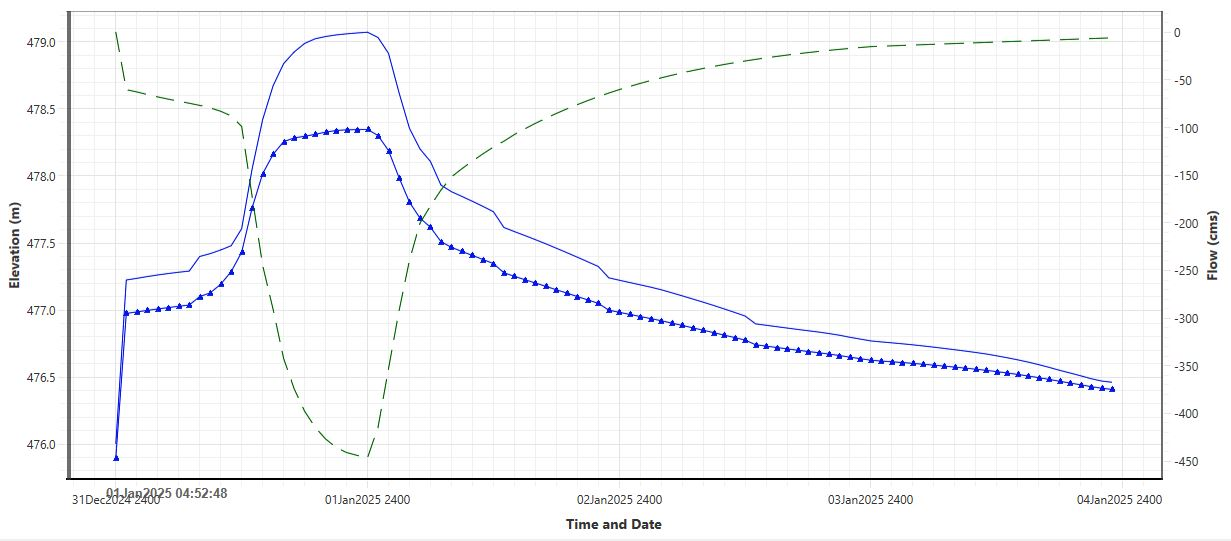
\includegraphics[scale=0.5]{immagini/flow_ponte_piave.JPG}
    \caption{Portata di deflusso transitata al di sotto del ponte nel fiume Piave, calcolata con la terza simulazione. Il plot della linea invertita è dovuto solamente al differente verso di disegno della linea di profilo.}
    \label{figure:flow_ponte_piave}
\end{figure}

\begin{table}[hbt]\centering
    \caption{\textcolor{red}{Valori numerici riferiti ai volumi di deflusso transitati attraverso le luci dei ponti dei rispettivi fiumi, a seconda della simulazione svolta. In tutti i casi, l'unità di misura è [1000 \unit{m^3}].}}
    \begin{tabular}{ccc}
    \toprule
    Simulazione & V. Boite & V. Piave \\
    \midrule
    1 & 39660.54 & 35555.61 \\
    2 & 39586.4 & 35551.91 \\
    3 & 39619.15 & 35518.3  \\
    \bottomrule
    \end{tabular}
    \label{table:flusso_ponti}
    \end{table}

La tabella \eqref{table:flusso_ponti} presenta dei valori che sono da contestualizzare, perché i casi sono diversi a seconda del fiume preso in considerazione.\\
Il volume trasportato dal fiume Piave dovrebbe rimanere costante per tutte le simulazioni (infatti il valore non varia molto), poiché a monte del proprio ponte non avvengono esondazioni che ne riducono la quantità transitata tra i piloni.\\
Per quanto riguarda il fiume Boite, si può notare una apprezzabile differenza, tra le diverse simulazioni, di volume transitato sotto il ponte. Questa differenza è dovuta all'esondazione che avviene verso l'abitato, a monte del ponte, che riduce il volume di passaggio sotto l'opera.

\subsection{Evento di esondazione}
Dai risultati delle simulazioni, risulta semplice notare il verificarsi di una esondazione del fiume nel centro abitato del paese di Perarolo di Cadore.\\
Ai fini di protezione civile, è importante conoscere i volumi esondati ed il tirante d'acqua che si genera nelle aree interessate.\\
Per fare ciò, è stato creato un profilo di studio lungo tutta l'arginatura che divide l'alveo del fiume e l'abitato del paese, che è stato chiamato ``profilo\textunderscore abitato".

\begin{figure}[H] \centering
    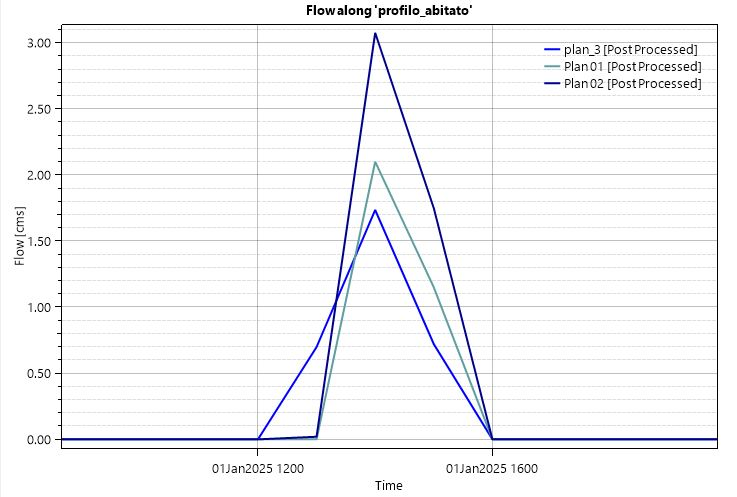
\includegraphics[scale=0.5]{immagini/flow_centro_abitato.JPG}
    \caption{Portata di flusso esondata nel centro abitato, rilevata mediante il ``profilo\textunderscore abitato".}
    \label{figure:flow_centro_abitato}
\end{figure}

\begin{figure}[H] \centering
    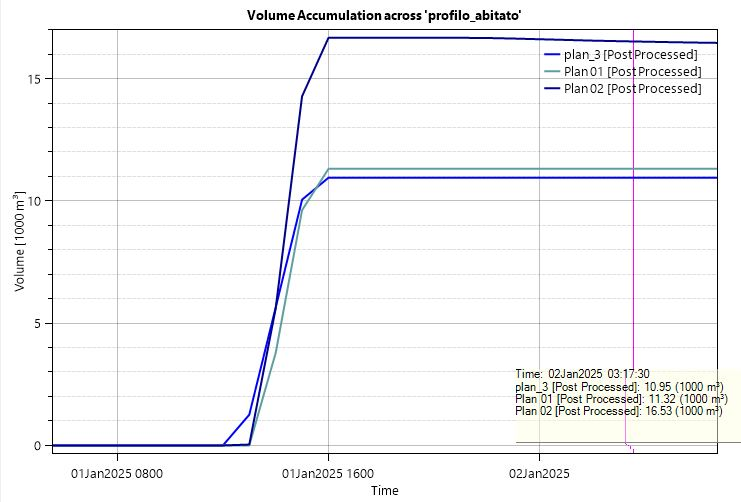
\includegraphics[scale=0.5]{immagini/volume_accumulation_centro_abitato.JPG}
    \caption{Volume cumulato di acqua esondata verso il centro abitato, rilevato mediante il ``profilo\textunderscore abitato".}
    \label{figure:volume_accumulation_centro_abitato}
\end{figure}

\begin{figure}[H] \centering
    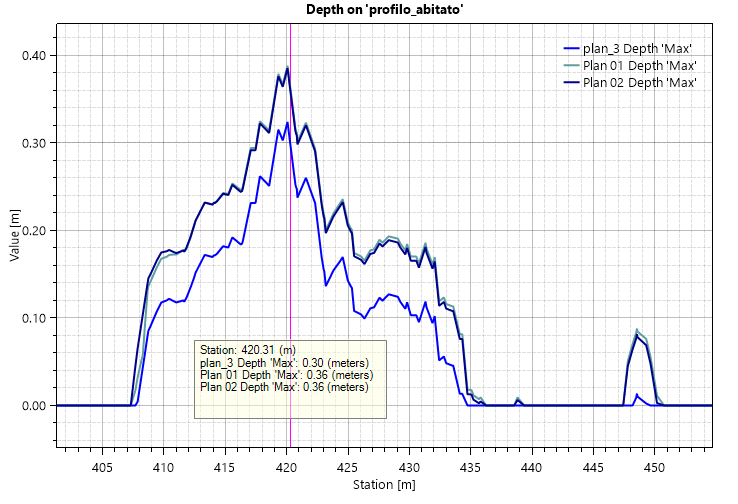
\includegraphics[scale=0.5]{immagini/depth_profilo_abitato.png}
    \caption{Profondità del tirante idraulico massimo sfiorata dalle arginature (rappresentate mediante il ``profilo\textunderscore abitato").}
    \label{figure:depth_profilo_abitato}
\end{figure}

Com'è possibile notare nel diagramma dei volumi cumulati, la condizione più gravosa per il sistema avviene nella seconda simulazione.\\
Nella tabella \eqref{table:risultati_arginatura} vengono riportati i principali parametri di esondazione, riferiti principalmente al rilievo mediante il profilo della zona d'abitato (ovvero sull'arginatura).\\
Sarebbe comunque possibile misurare la profondità del tirante idraulico che si creerebbe nell'abitato, in modo da poter svolgere dei ragionamenti su eventuali allagamenti.\\
L'altezza del tirante idraulico che si genera nell'arginatura è un fattore importante perché, come indicato dal Distretto di Bacino della Alpi Orientali, permette di prevedere il rischio che si formino eventuali brecce arginali (se in forma continuata per un certo tempo); tale evento andrebbe a peggiorare l'evento di esondazione inizialmente stimato.

\begin{table}[hbt]\centering
    \caption{\textcolor{red}{Valori numerici riferiti all'evento di esondazione del tratto fluviale verso l'abitato. I valori di tirante idraulico e di portata al picco sono riferiti all'arginatura, mentre il volume totale può essere considerato per tutta l'area esondata.}}
    \begin{tabular}{cccc}
    \toprule
    Sim. & Tirante idraulico [m] & Volume [1000 \unit{m^3}] & Portata al picco [\unit{m^3/s}] \\
    \midrule
    1 & 0.36 & 11.32 &   2.10\\
    2 & 0.36 & 16.53 & 3.07  \\
    3 & 0.30 & 10.95 & 1.74  \\
    \bottomrule
    \end{tabular}
    \label{table:risultati_arginatura}
    \end{table}

Com'è possibile capire leggendo la tabella, il caso più gravoso per la comunità adiacente al fiume è prodotto dalla seconda simulazione, ovvero quella con un indice di scabrezza intermedio.

\subsection{Aree di pericolo}
Al fine di valutare la pericolosità di un'area, occorre innanzitutto considerare la tipologia di evento in atto; i criteri con cui è possibile differenziare un evento sono disponibili all'interno della ``Relazione generale" del PGRA \cite{rel_gen_pgra}.\\
E' necessario far presente che i risultati della simulazione non sono vincolanti per la delimitazione delle aree di pericolo; infatti, il tecnico, in forma cautelativa, può legittimamente decidere di aumentare le aree a maggiore tutela.\\
Essendo che l'evento di piena ha un tempo di ritorno di 215 anni, la probabilità di accadimento viene considerata ``medio-bassa".\\
Successivamente, al fine di discretizzare l'attribuzione della pericolosità ad un'area, viene applicata la matrice di BUWAL, che va ad interpolare la probabilità d'accadimento e l'intensità dell'evento (che a sua volta è in funzione del tirante idraulico e della velocità del flusso).\\
Infatti, l'Autorità di bacino per il Distretto delle Alpi Orientali ha definito 3 classi di intensità, che sono state riportate inizialmente nel paragrafo sulle normative presenti \eqref{section:normative}.\\
Per un evento di questo tempo di ritorno, il PGRA prevede che la classificazione del pericolo prenda valore P1 o P3 (rispettivamente- il minimo ed il massimo attribuibile ad un'area).\\

\begin{figure}[H] \centering
    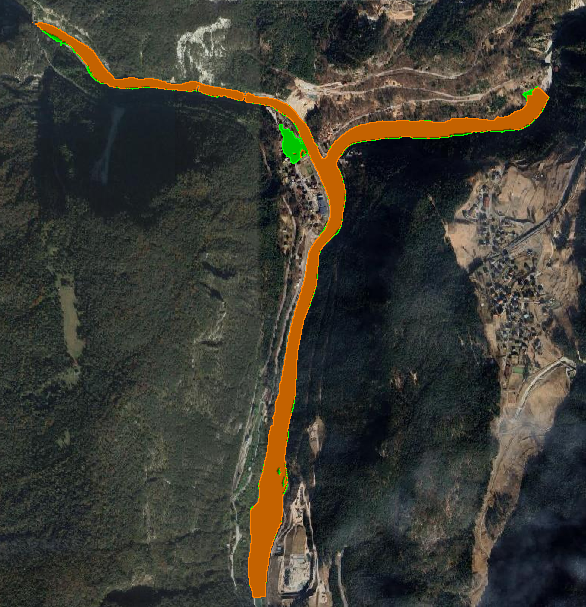
\includegraphics[scale=0.5]{immagini/aree_pericolo_1.png}
    \caption{Aree di pericolo ricavate dalla simulazione 1.}
    \label{figure:aree_pericolo_1}
\end{figure}

\begin{figure}[H] \centering
    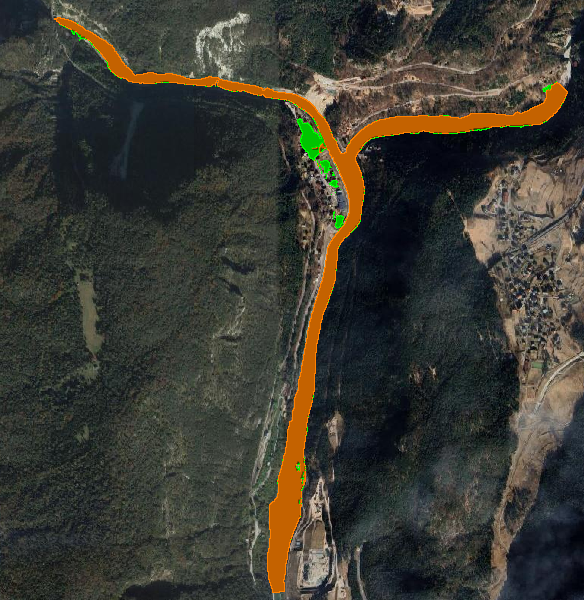
\includegraphics[scale=0.5]{immagini/aree_pericolo_2.png}
    \caption{Aree di pericolo ricavate dalla simulazione 2.}
    \label{figure:aree_pericolo_2}
\end{figure}

\begin{figure}[H] \centering
    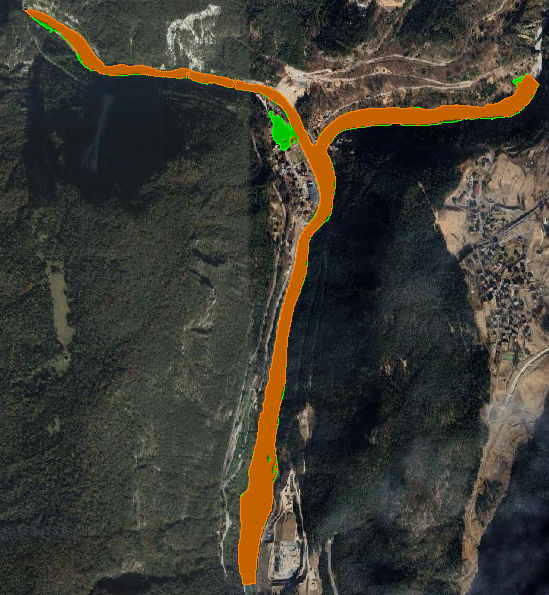
\includegraphics[scale=0.5]{immagini/aree_pericolo_3.png}
    \caption{Aree di pericolo ricavate dalla simulazione 3.}
    \label{figure:aree_pericolo_3}
\end{figure}

\begin{figure}[H] \centering
    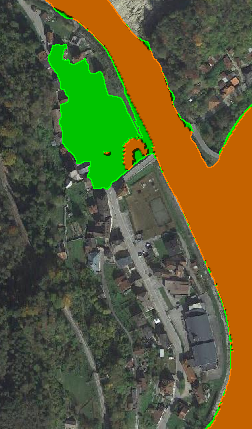
\includegraphics[scale=0.5]{immagini/part_aree_pericolo_1.png}
    \caption{Aree di pericolo ricavate dalla simulazione 1 (particolare dell'abitato).}
    \label{figure:part_aree_pericolo_1}
\end{figure}

\begin{figure}[H] \centering
    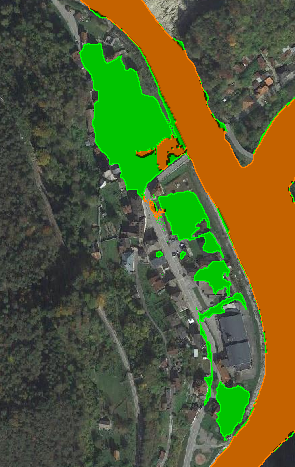
\includegraphics[scale=0.5]{immagini/part_aree_pericolo_2.png}
    \caption{Aree di pericolo ricavate dalla simulazione 2 (particolare dell'abitato).}
    \label{figure:part_aree_pericolo_2}
\end{figure}

\begin{figure}[H] \centering
    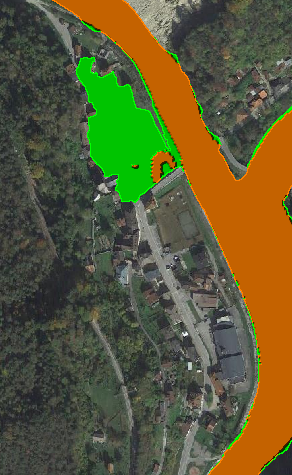
\includegraphics[scale=0.5]{immagini/part_aree_pericolo_3.png}
    \caption{Aree di pericolo ricavate dalla simulazione 3 (particolare dell'abitato).}
    \label{figure:part_aree_pericolo_3}
\end{figure}

Le aree considerate a pericolo P3 sono rappresentate in arancione, mentre quelle valutate a rischio basso sono di colore verde; questa scelta cromatica risulta concorde con quella generalmente adottata nelle cartografie ufficiali del Distretto di Bacino.\\
In tutti e tre i scenari, ovviamente, le aree dell'alveo sono considerate come di pericolo P3, dato l'elevato tirante idraulico e la velocità sostenuta; nel contempo, varia la determinazione di pericolo per le zone dell'abitato del paese. Nel caso in cui l'esondazione fosse maggiore, per esempio, con molta probabilità la strada che porta al ponte verrebbe considerata ad elevato pericolo, poiché in quel tratto la velocità del flusso sarebbe elevata.\\
Infatti, andando a comparare le figure \eqref{figure:part_aree_pericolo_1}\eqref{figure:part_aree_pericolo_2}\eqref{figure:part_aree_pericolo_3}, è possibile notare come la prima e la terza simulazione producano all'incirca la stessa esondazione, mentre la seconda simulazione genera una maggiore area allagata. Questi risultati sono concordi con quanto riportato nella tabella \eqref{table:risultati_arginatura}.